\documentclass{llncs}
\usepackage{graphicx}
\begin{document}

\title{Matching de Formes}

\author{Julien ALTIERI, Benoit SEGUIN, Frederic WILHELM\institute{Ecole Polytechnique, X2008}}



\maketitle

\begin{abstract}
Le \textit{matching de formes} est un probl\`eme r\'ecurrent de g\'eom\'etrie algorithmique. Il s'agit d'une part d'\'evaluer la \textit{proximit\'e g\'eom\'etrique} de deux maillages ind\'ependamment de ces maillages, et d'autre part de trouver une \textit{transformation rigide} qui envoie l'un sur l'autre, de mani\`ere optimale. Le d\'efi consiste donc à extraire des propri\'et\'es g\'eom\'etriques \textit{intrins\`eques} de l'objet, ce que nous faisons en exploitant le \textit{tenseur de courbure}. \textbf{suite \`a expliquer pour la transformation rigide}.
\end{abstract}

\section{Introduction, motivation, ...}
Nous souhaitions au d\'epart d\'evelopper un jeu de sculpture, avec des formes \`a reproduire. Cet objectif nous a naturellement conduit \`a devoir \'evaluer un score de proximit\'e, et donc au matching de forme.


%si on veut faire une figure (ceci est un commentaire => retirer les % pour decommenter)
%\begin{figure}
%\center
%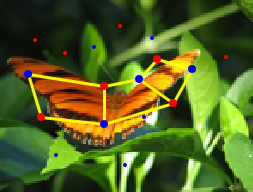
\includegraphics[bb=0 0 253 192, width=5cm]{relevantinformation.png}
%\caption{un commentaire ?}
%\end{figure}




\section{La m\'ethode employ\'ee}
Voici un exemple~\cite{rugis} pour faire une citation.


\section{\'Evaluer le tenseur de courbure}


\section{Comparer deux courbures}


\section{Organisation du code}


\section{Conclusion}


\bibliographystyle{plain}
\bibliography{exampleProject}
\end{document}


